\section{Operational Semantics}


\begin{frame}
\frametitle{Operational Semantics}
\framesubtitle{Stages}
The semantics are presented in two stages:
\begin{itemize}
    \item the local level: captures the sequential behaviour of one thread
    \item the global level : deals with concurrent threads and lock handling
\end{itemize}


\end{frame}

\begin{frame}
\frametitle{Operational Semantics}
\framesubtitle{Local Steps}

At the local level, a configuration is 
\begin{align*}
    \tag{Local Configuration}
    \sigma \vdash e,
    \text{where} ~\sigma~ \text{is the heap}
\end{align*}

and it represents the mutable state of the program shared between all threads.
\newline \\
$\sigma$ contains the allocated objects and locks.

\begin{equation}
    \tag{Local Reduction Step}
    \sigma \vdash e \longrightarrow \sigma' \vdash e'
\end{equation}
\end{frame}

\begin{frame}
\frametitle{Operational Semantics}
\framesubtitle{Local Steps}
Each lock has an identity and is either free, or taken by one particular thread. 

\begin{itemize}
    \item the value 0 represents a lock which is not held by any thread
    \item $p(n) \forall n \ge 1$ express a lock hold by thread $p$, n times 
\end{itemize}
\end{frame}

\begin{frame}
\frametitle{Operational Semantics}
\framesubtitle{Local Semantics}
\begin{figure}[h]
    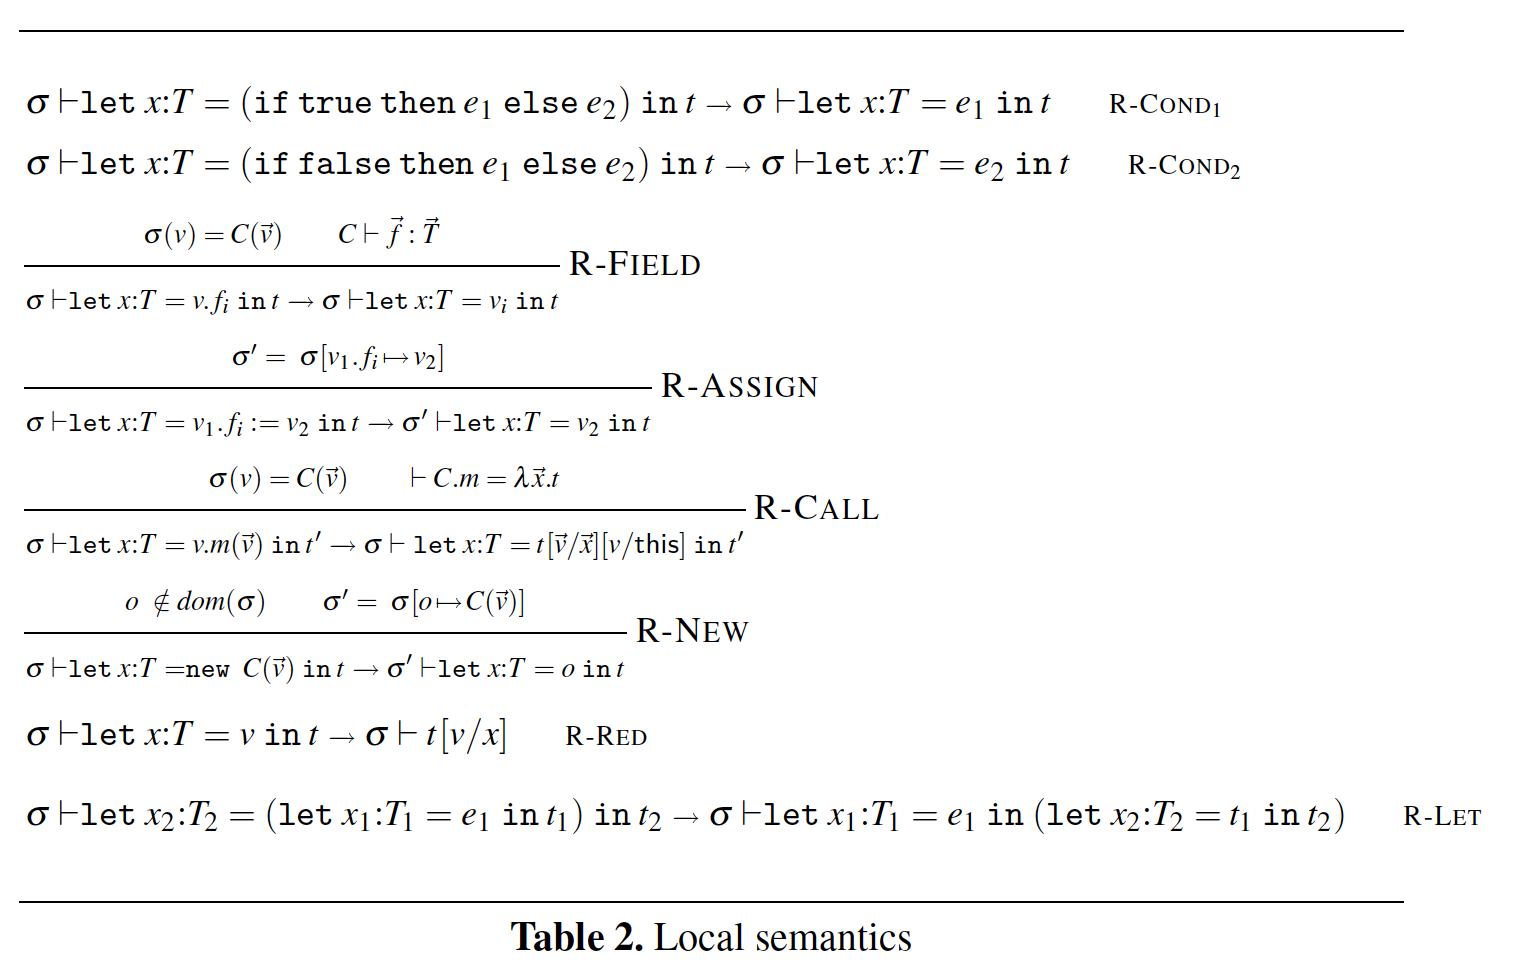
\includegraphics[width=10cm]{figures/local.png}
    \label{fig::local::semantics}
\end{figure}
\end{frame}

\begin{frame}
\frametitle{Operational Semantics}
\framesubtitle{Global Steps}
The global steps concern more than one sequential thread, and the thread identity plays a primary role. 
\newline \\
A global configuration consists of 
\begin{itemize}
    \item a shared heap $\sigma$ which contains the “passive” data part
    \item a set of processes P which contains the "active" part
\end{itemize}
\end{frame}


\begin{frame}
\frametitle{Operational Semantics}
\framesubtitle{Global Configuration}
\begin{equation}
    \tag{Global Configuration \& Step}
    \sigma \vdash P, \sigma \vdash P \longrightarrow \sigma' \vdash P' 
\end{equation}
where the processes P follow the grammar
\begin{center}
\begin{minipage}{0.8\linewidth}
\begin{grammar}
<P> $\coloncolonequals 0$ | $P \| P$ 
    | $p\langle t \rangle$
\end{grammar}
\end{minipage}
\end{center}
where
\begin{itemize}
    \item $0$ represents the empty process (neutral element)
    \item $P_1 \| P_2$ represents a parallel composition of processes (associative and commutative operation)
    \item $p\langle t \rangle$ represents a process or named thread, where $p$ is the process identity and $t$ the thread being executed
\end{itemize}
\end{frame}


\begin{frame}
\frametitle{Operational Semantics}
\framesubtitle{Processes}

\begin{center}
$P$: thread names $\longrightarrow$ expressions \\
$dom(P)$ = \{name of $t$ | $\forall t$ thread running in $P$\}
\end{center}
\begin{align}
P_1 \| P_2 ~\text{iff}~ dom(P_1) \cap dom(P_2) = \emptyset
\end{align}
\end{frame}

\begin{frame}
\frametitle{Operational Semantics}
\framesubtitle{Global Semantics (I)}
\begin{figure}[h]
    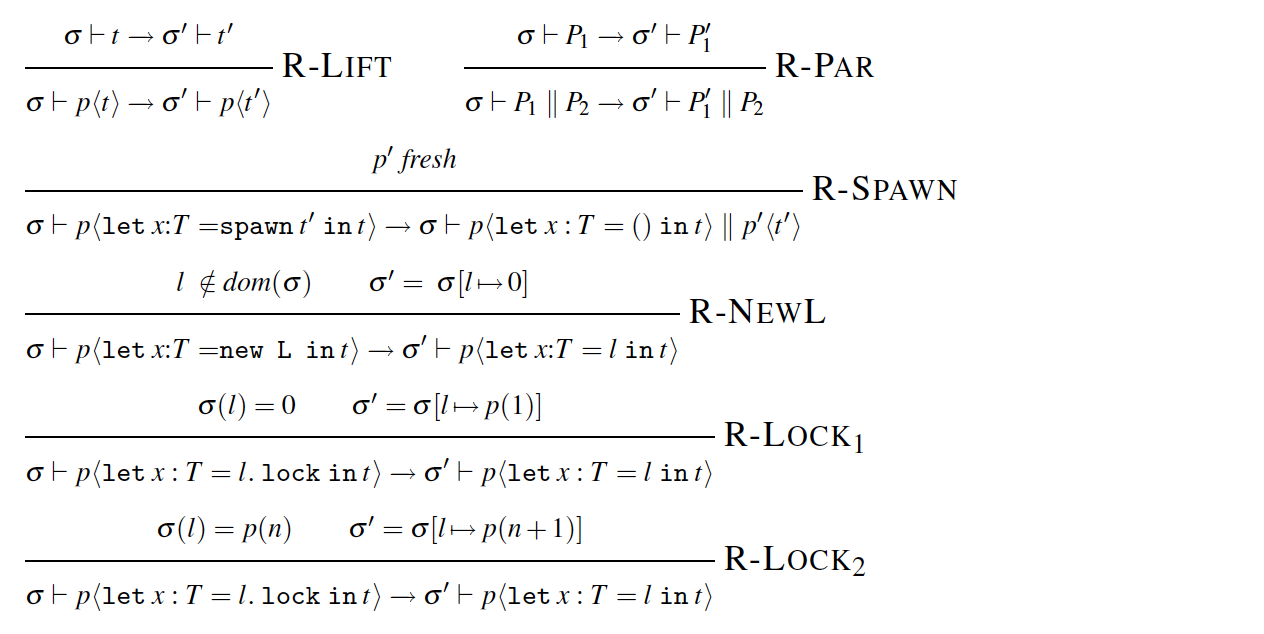
\includegraphics[width=10cm]{figures/global_a.png}
    \label{fig::global_a::semantics}
\end{figure}
\end{frame}


\begin{frame}
\frametitle{Operational Semantics}
\framesubtitle{Global Semantics (II)}
\begin{figure}[h]
    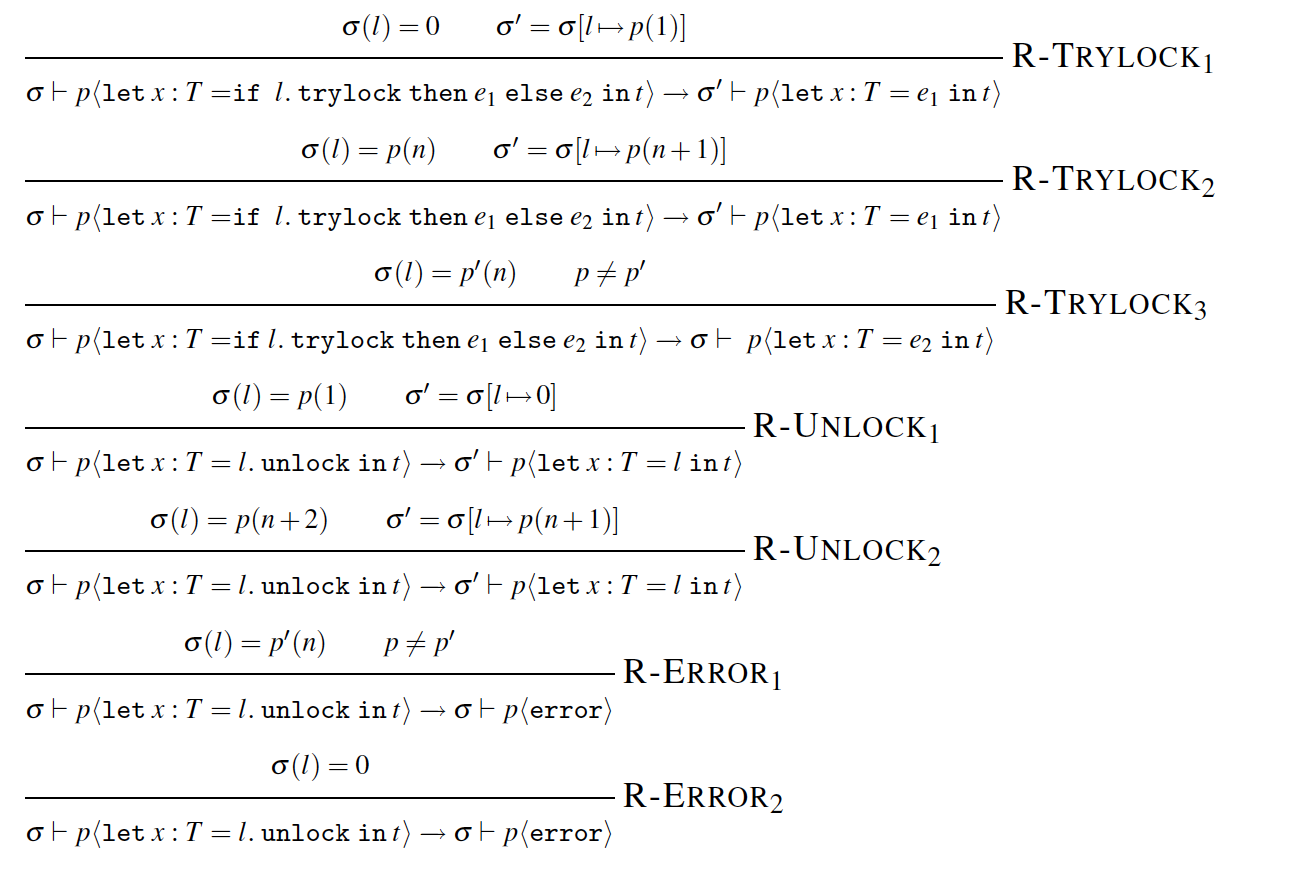
\includegraphics[width=10cm]{figures/global_b.png}
    \label{fig::global_a::semantics}
\end{figure}
\end{frame}